\clearpage
\section{Обсуждение}

\subsection{Анализ всех найденных видов}

У всех проанализированных видов размер второго экзона из ``консервативной кассеты`` равен 37 нуклеотидам, в то время как размер первого экзона варьирует в различных группах.
На рисунке~\ref{fig:Protostomia_exon} показано распределение длины первого экзона из ``кассеты`` для Protostomia.

\begin{figure}[h] % here, top, bottom, page
    \centering
    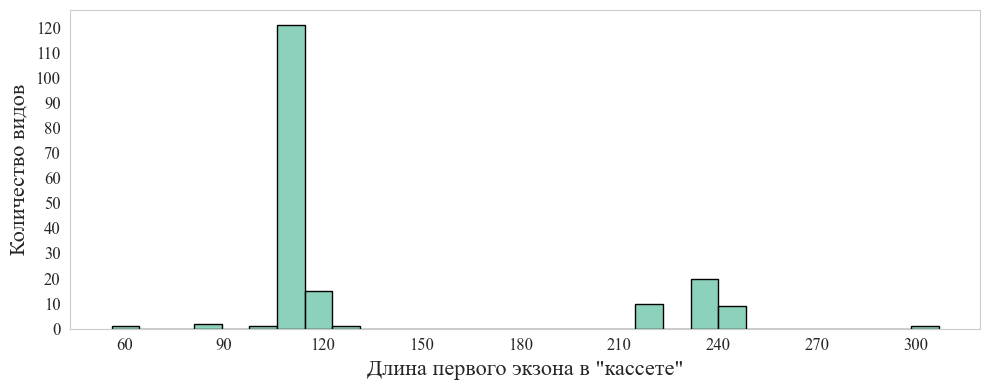
\includegraphics[width=0.9\textwidth]{images/Protostomia_exon}
    \caption{Распределение длины первого экзона из ``консервативной кассеты``.}
    \label{fig:Protostomia_exon}
\end{figure}

Для Ecdysozoa и Cnidaria первый экзон как правило размером 110 нуклеотидов, но встречаются и исключения.
У Spiralia размер этого экзона гораздо больше и чаще всего составляет 239 нуклеотидов.
По данному отличию и встречающимся уникальным вариантам размера экзона требуется углубленное исследование.

У Deuterostomia размер первого экзона в абсолютном большинстве случаев (171 из 172 исследованных видов) составляет 110 нуклеотидов, что также характерно и для млекопитающих.

Длина участка внутри интрона до стоп-кодона, как и длина самого интрона, варьирует в более широких пределах в разных группах.
Тем не менее внутри отдельных групп, например Lepidosauria (таблица~\ref{tab:Lepidosauria} в приложении), наблюдается высокая степень консервативности обоих параметров.

Также встречаются виды, у которых происходит частичная или даже полная трансляция ``кассетного`` интрона, потому что в нем не встречается преждевременный стоп-кодон.
Например, таким видом является давно известный \textit{Caenorhabditis elegans}, у которого преждевременный стоп-кодон встречается в одном из экзонов после ``кассетного`` интрона.
В данном исследовании были найдены еще 2 вида, у которых интрон полностью считывается: Aves - \textit{Vidua chalybeata}, Paraneoptera - \textit{Rhopalosiphum maidis}.
Упомянутые виды также требуют тщательного изучения.


\subsection{Анализ группы Actinopterygii}

Данная группа организмов была исследована более подробно по перечисленным ранее причинам.
Внутри группы размеры первого и второго экзона из ``консервативной кассеты`` для всех исследованных видов составляют 110 и 37 нуклеотидов, соответственно.
Длина участка внутри интрона до стоп-кодона у большинства видов составляет 22 нуклеотида (39 из 72 исследованных в работе).
Размер ``кассетного`` интрона варьирует от 1702 до 4202 нуклеотидов (в среднем 2705).

Анализ ``сайтов силы сплайсинга``~\ref{fig:Actinopterygii_maxentscan} говорит о том, что практически у всех видов данный интрон успешно вырезается сплайсосомой.
Учитывая большую выборку видов, взятую для анализа, было принято решение ориентироваться на эмпирическую интерпретацию результатов, которая выглядит следующим образом:

\begin{spacing}{0.5}
\begin{itemize}
    \item 0–3: слабый сайт сплайсинга
    \item 3–6: умеренный сайт сплайсинга
    \item >6: сильный сайт сплайсинга
\end{itemize}
\end{spacing}

Так как у большинства видов значение MaxEntScan score больше или около 6, был сделан вывод, высказанный выше.
Соответственно, невырезание сплайсосомой как минимум у данной группы не является причиной альтернативного сплайсинга с сохранением ``кассетного`` интрона.

В связи с этим и было принято решение о поиске консервативных мотивов внутри ``кассетного`` интрона.
Несмотря на то, что на рисунке~\ref{fig:Actinopterygii_meme} представлено 5 найденных мотивов, их количество может быть больше, потому что данное значение мотивов было ограничением запуска MEME Suite.
Учитывая высокую степень сходства начала 2-го найденного мотива с консенсусной последовательностью CTE из рисунка~\ref{fig:CTE_consensus}, можно предположить сохранение интрона благодаря этой и возможно другим структурам внутри интрон-содержащего транскрипта (рисунок~\ref{fig:Chanos_chanos_2nd_structure}).

Проведенное множественное выравнивание на рисунке~\ref{fig:Actinopterygii_alignment_ruler} говорит о высокой степени консервативности как кодирующих участков (левый и правый крайние части диаграммы под выравниванием), так и некоторых участков внутри интрона (центр диаграммы под выравниванием).
Филогенетическое древо (рисунок~\ref{fig:Actinopterygii_tree}), построенное по результатам выравнивания, несмотря на наличие ``кассетного`` интрона в последовательности, использованной для его построения, успешно разделяет виды на таксоны более высокого ранга - Otomorpha и Euteleosteomorpha.

Остальные группы, не включенные в подробный анализ, требуют его проведения.